\documentclass{article}
\usepackage{amsmath,amsfonts,amsthm,amssymb,amsopn,bm}
\usepackage[margin=.9in]{geometry}
\usepackage{graphicx}
\usepackage{url}
\usepackage[usenames,dvipsnames]{color}
\usepackage{fancyhdr}
\usepackage{multirow}
\usepackage{listings}
\usepackage{hyperref}

\definecolor{keywords}{RGB}{255,0,90}
\definecolor{comments}{RGB}{0,0,113}
\definecolor{red}{RGB}{160,0,0}
\definecolor{green}{RGB}{0,150,0}
 
\lstset{language=Python, 
        basicstyle=\ttfamily\tiny, 
        keywordstyle=\color{keywords},
        commentstyle=\color{comments},
        stringstyle=\color{red},
        showstringspaces=false}

\newcommand{\field}[1]{\mathbb{#1}}
\newcommand{\1}{\mathbf{1}}
\newcommand{\E}{\mathbb{E}} 
\newcommand{\Z}{\mathbb{Z}} 
\renewcommand{\P}{\mathbb{P}}
\newcommand{\R}{\field{R}} % real domain
% \newcommand{\C}{\field{C}} % complex domain
\newcommand{\F}{\field{F}} % functional domain
\newcommand{\T}{^{\textrm T}} % transpose
\def\diag{\text{diag}}

%% operator in linear algebra, functional analysis
\newcommand{\inner}[2]{#1\cdot #2}
\newcommand{\norm}[1]{\left\|#1\right\|}
\newcommand{\twonorm}[1]{\|#1\|_2^2}
% operator in functios, maps such as M: domain1 --> domain 2
\newcommand{\Map}[1]{\mathcal{#1}}
\renewcommand{\theenumi}{\alph{enumi}} 

\newcommand{\Perp}{\perp \! \! \! \perp}

\newcommand\independent{\protect\mathpalette{\protect\independenT}{\perp}}
\def\independenT#1#2{\mathrel{\rlap{$#1#2$}\mkern2mu{#1#2}}}
\newcommand{\vct}[1]{\boldsymbol{#1}} % vector
\newcommand{\mat}[1]{\boldsymbol{#1}} % matrix
\newcommand{\cst}[1]{\mathsf{#1}} % constant
\newcommand{\ProbOpr}[1]{\mathbb{#1}}
\newcommand{\points}[1]{\small\textcolor{magenta}{\emph{[#1 points]}} \normalsize}
\date{{}}

\setlength\parindent{0px}

\begin{document}
\title{Homework \#2}
\author{\normalsize{Winter 2020, STATS 509}\\
\normalsize{Dino Bektesevic}}
\maketitle

\section*{Problem 1}
\begin{enumerate}
	\item in this case k=1 so the winnings can only be 0 or 2/3, i.e. $X_1=\{0, 2/3\}$. The probability of each coin toss is 1/2. We can write the pmf function as:
	$$f(x) = \begin{cases} 
	        1/2 &\mbox{if } x \in X_1 \\
            0 & \mbox{if } x \notin X_1 
        \end{cases} 
    $$
    essentially saying that the probability of seeing random variable $x$ be either win or lose is 50 percent. the cumulative distribution function, i.e. cdf, is given by $F_X(x) = P(X\leq x) = \sum_i p(x_i)$. In our case this boils down to three cases, corresponding to the two mass points - a win or no win:
	$$F(x) = \begin{cases} 
	        0 &\mbox{if } x < 0 \\
	        1/2 &\mbox{if } 0 \leq x \leq 2/3 \\
            1 & \mbox{if } x > 2/3 
        \end{cases} 
    $$

    \item in case of k=2 there are 4 different winnings $X_2=\{0, 2/3, 2/9, 8/9\}$ corresponding to four outcome cases (where ordering matters) $x=\{tt, ht, th, hh\} = \{\mbox{0+0}, \mbox{2/3+0}, \mbox{0+2/9}, \mbox{2/3+2/9}\}$. The probability of each outcome is 1/4 because these are two independent events each with probability of 1/2. Written down:
    $$f(x) = \begin{cases} 
	        1/4 &\mbox{if } x \in X_2 \\
            0 & \mbox{if } x \notin X_2 
        \end{cases} 
    $$
	Similarly there are now 5 cases corresponding to the 4 mass points in the cdf:
	$$F(x) = \begin{cases} 
	        0 &\mbox{if } x < 0 \\
	        0.25 &\mbox{if } 0\leq x \leq 2/9 \\
            0.5  & \mbox{if } 2/9 < x \leq 2/3 \\
            0.75 & \mbox{if } 2/3 < x \leq 8/9 \\
            1 & \mbox{if } x > 8/9
        \end{cases} 
    $$
	
	\newpage
	\item I run a million simulations counting up all the winnings from each toss in each simulation in Python.
	\begin{center}
    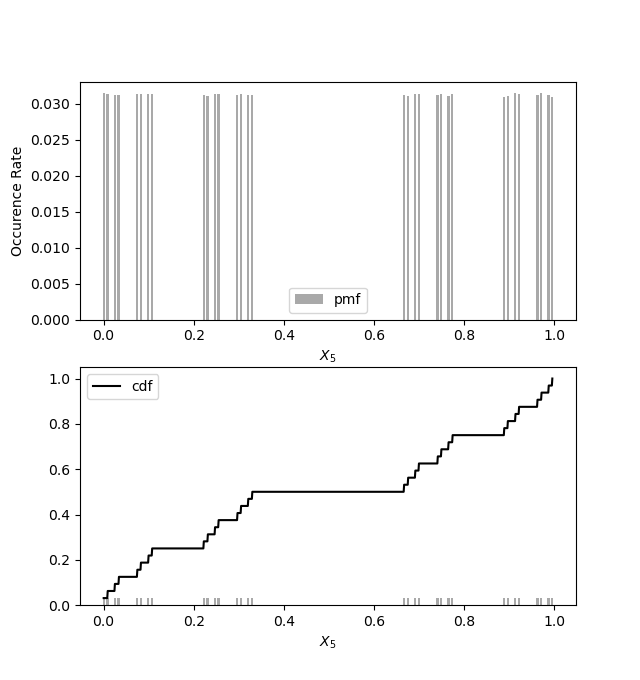
\includegraphics[width=2.5in]{STATS509/HW2/HW2Figures/problem1c.png}
    \end{center}
    \lstinputlisting[language=Python]{HW2Code/HW2_Problem1.py}
\end{enumerate}


\newpage
\section*{Problem 2}
\begin{enumerate}
	\item Problem states that the events are overlapping sets ($P(A\cap B) =0.06$
	\item From 2nd axiom of probability: $P(A\cup B) = P(A) + Pr(B) - P(A\cap B) \rightarrow P(B) = P(A\cup B)  - P(A) + P(A\cap B) = 0.2$
	\item Since we know $P(A)=0.3$ and have calculated $P(B)=0.2$ we can verify $P(A)P(B)=0.06=P(A\cap B)$ and conclude that yes, they could be independent.
\end{enumerate}


\section*{Problem 3}
We can start with 2nd axiom of probabilities again $P(A\cup B) = P(A) + Pr(B) - P(A\cap B)$ and notice that because Z takes only integer values we have $P(Z<1 \cap Z\geq 0) = P(Z=0)$ which is exactly what we are looking for. Additional information we have is that $P(Z<1 \cup Z\geq 0) = 1$ since the union spans the entire $\Z$, i.e. the domain of the random variable Z.
\begin{align*}
P(A\cup B) =& P(A) + Pr(B) - P(A\cap B) \\
P(Z<1 \cup Z\geq 0) =& P(Z<1) + P(Z\geq 0) - P(Z=0) \\
P(Z=0) =& P(Z<1) + P(Z\geq 0) - P(Z<1 \cup Z\geq 0) \\
P(Z=0) =& a + b - 1
\end{align*}

\newpage
\section*{Problem 4}
\begin{enumerate} 
    \item We have a system of equations:
    \begin{align*}
    P(A\cup B) &= r = P(A) + P(B) - P(A\cap B) \\
    P(A\cup C) &= s = P(A) + P(C) - P(A\cap C) \\
    P(A\cup B\cup C) &\leq 1 \geq P(A) + P(B) + P(C) - P(A\cap B) - P(A\cap C) - P(B \cap C) - P(A\cap B \cap C) \\
    \end{align*}
    Multiplying the first two with a -1 and adding them we have:
    \begin{align*}
    -r - s &= -2P(A) - P(B) + P(A\cap B) + P(A\cap C) \\
    1 &\geq P(A) + P(B) + P(C) - P(A\cap B) - P(A\cap C) - P(B \cap C) + P(A\cap B \cap C) \\
    \end{align*}
    Maximizing the $P(A)$ is assuming probabilities add up to 1, since we are looking for extrema that's what we do. Adding what's left together:
    \begin{align*}
    1-r-s &= -P(A) - P(B \cap C) + P(A\cap B \cap C) \\
    P(A) &= r + s + P(A\cap B \cap C) - P(B \cap C) - 1
    \end{align*}
    \item Following above, we have:$ P(A) = r + s + t -1 - P(B \cap C)$.
\end{enumerate}

Mathematically I was unable to further resolve the problem. Attending office hours a proverb was shared with me about a dog that barks but isn't, but I didn't understand it - refer to professor Thomas for details. However, it makes sense that since  $P(A) \leq P(A\cup B)$ and $P(A) \leq P(A\cup C)$, by implication the maximal probability for both sections of the problem is limited to $\min{(s, r)}$ . For a) part of the problem there is nothing that really limits our lower bound so we must say $0 \leq P(A) \leq \min{(s, r)}$ while in the b) part of the problem we can say $t \leq P(A) \leq \min{(s, r)}$ since, by implication again, $P(A)\geq P(A\cap B\cap C)$.

\newpage
\section*{Problem 5}
\begin{enumerate}
	\item \addtocounter{enumi}{3} b. c. \begin{table}[h]
            \begin{tabular}{cc|c|c|c}
            $t_1$ & $t_2$  & avg($Y_T$) & avg($Y_C$) & avg($Y_T$)-avg($Y_C$)\\ \hline
            1 & 2 & 6   & 4.5 & 1.5 \\
            1 & 3 & 4   & 6   & -2 \\
            1 & 4 & 5.5 & 3.5 & 2 \\ 
            2 & 1 & 6   & 4.5 & 1.5 \\
            2 & 3 & 8   & 5   & 3 \\
            2 & 4 & 9.5 & 2.5 & 7 \\
            3 & 1 & 4   & 6   & -2 \\
            3 & 2 & 8   & 5   & 3 \\
            3 & 4 & 7.5 & 4   & 3.5 \\
            4 & 1 & 5.5 & 3.5 & 2 \\
            4 & 2 & 9.5 & 2.5 & 7 \\
            4 & 3 & 7.5 & 4 & 3.5
            \end{tabular}
        \end{table}
    \item The average of the differences of hypothetical experiments is the mean value of the last column, i.e. $2.5$.
    \item The average of given $<Y_T>=6.75$ and the average of given $<Y_C>=4.25$, this their difference is again $2.5$
    \item The average differences are the same. This is the basis on which medical randomized trials are based - it is expected that the difference of averages of the two groups match the averages of individuals.
\end{enumerate}



\newpage
\section*{Problem 6}
\begin{enumerate}
	\item The probability of selecting a non-diseased person out of a group of $n$ people, $k$ of which are diseased, on our first pick is $1 - k/n$, on the second pick (assuming we picked a healthy individual) $1-k/(n-1)$
	$$P = \left(1 - \frac{k}{n}\right) \left(1 - \frac{k}{n-1}\right) \dots \left(1 - \frac{k}{n-m}\right) $$
	where we chose a total of $m$ times, i.e. people. Reducing:
	\begin{align*}
    P &= \left(\frac{n-k}{n}\right) \left(\frac{n-k-1}{n-1}\right) \dots \left(\frac{n-k-m}{n-m}\right) \\
      &= \frac{(n-k)!(n-m)!}{n!(n-k-m)!} \\
    \end{align*}
    Probability that our pick contains a diseased person, i.e. the probability that a pick of $m$ random people from $n$ sample of people containing $k$ diseased people is, is the complement of the above probability:
    $$P = 1- \frac{(n-k)!(n-m)!}{n!(n-k-m)!}$$
    \item \addtocounter{enumi}{1} c.
        \begin{lstlisting}[language=Python]
def smallestSampleSizeWithP(k, n, Ptresh=0.95):
    i, P = 0, 1
    while True:
        P *= (1 - k / (n - i))
        i += 1
        if 1 - P >= Ptresh:
            return i, 1-P

print("m = {0}; at least 1 diseased P = {1}".format(*smallestSampleSizeWithP(20, 1000)))
print("m = {0}; at least 1 diseased P = {1}".format(*smallestSampleSizeWithP(200, 10000)))

>>> m = 138; at least 1 diseased P = 0.9502553198035257
>>> m = 148;; at least 1 diseased P = 0.9508276450580865
        \end{lstlisting}
    
    
    \item If we were to redo the first problem with replacement the probability of selecting a healthy individual would just be $(1-k/n)$ for each pick, rendering the probability of selecting only healthy people after $m$ picks $P=(1-k/n)^m$. This is implied by the hint. Putting in values from part c, and using the complement to recover the probability that we picked at least 1 diseased person:
    \begin{align*}
    P =& 1 - \left(1-\frac{k}{n}\right)^m \\
    0.95 =& 1 - \left(1-\frac{200}{10000}\right)^m \\
    m =& 148.284
    \end{align*}
    which is reasonably close to our numerically solved answer in c, keeping in mind that m actually has to be integer. The problem here is reducing the binomial distribution to that probability, which can be written down as
    $$P = {n \choose k} p^k (1-p)^{n-k}$$
    setting $n=k=m$ we can rewrite:
    $$P = {m \choose m} p^m (1-p)^{m-m} = p^m$$
    and since from earlier we know that success probability of each trial pick is $p=1-n/k$ we write the probability of choosing m consecutive non-deseased individuals as:
    $$P = \left(1-\frac{k}{n}\right)^m$$
    the complement of which gives us the expression we started this problem from. While I do not have good motivation for setting the population to the size of the sample, while designating them all to be diseased (a given eventuality in current circumstances) there is motivation to use sampling with replacement in circumstances where our population is very large. The probability of picking the same person twice tends towards 0 as the population size tends towards infinity.
\end{enumerate}




\newpage
\section*{Problem 7}
Considering the following cases:
\begin{enumerate}
	\item A = \{X=1\}
	\item B = \{X=2\}
	\item C = \{X $\leq$ 3\}
	\item D = \{X is even\}
	\item E = \{1 $<$ X $<$ 5\}
	\item F = $C\cup D$
	\item G = $C\cap D$
\end{enumerate}
and Bernoulli, Uniform and Binomial distributions with the following expressions, in order:
\begin{align*}
f(x) &= p^x(1-p)^{1-x} \text{ for } x={0,1} \text{ and } 0 \text{ elsewhere } \\
f(x) &= \frac{1}{N} \text{ at } x_i \text{ and } 0 \text{ elsewhere } \\
f(x) &= \frac{n!}{x!(n-x)!}p^x(1-p)^{n-x} \text{ for } x={0,\dots,n} \text{ and } 0 \text{ elsewhere }
\end{align*}
we have that for specific cases of:
\begin{enumerate}
	\item Bernoulli with parameter $p=0.4$, the following results for each case:
	\begin{enumerate}
    	\item 0.4
    	\item 0
    	\item 1
    	\item 0.6 (when treating 0 as even)
    	\item 0
    	\item 1
    	\item 0.6
    \end{enumerate}
    \item Discrete uniform with parameter $N=9$, the following results for each case:
	\begin{enumerate}
    	\item 1/9
    	\item 1/9
    	\item 3/9
    	\item 4/9
    	\item 3/9
    	\item 6/9
    	\item 1/9
    \end{enumerate}
    \item Binomial with parameter $n=2$ and $p=0.4$, the following results for each case:
	\begin{enumerate}
    	\item 0.48
    	\item 0.16
    	\item 1
    	\item 0.52
    	\item 0.16
    	\item 1
    	\item 0.52
    \end{enumerate}
\end{enumerate}





\end{document}
